\subsection{Telecommunication}


\begin{frame}{Telecommunication}{Line-Of-Sight}
  \begin{columns}[T]
    \begin{column}{.5\textwidth}
      \begin{block}{}
        \begin{itemize}
          \item {At high frequencies (above 30MHz) the ability to see the antenna roughly corresponds to the ability of receive the radio signal.}
          \item {Radio Horizon: Furthest possible point of propagation.}
          \item {OBS: Altitude with respect to the WGS84 datum.}
        \end{itemize}
      \end{block}
    \end{column}
    \begin{column}{.5\textwidth}
      \begin{figure}
        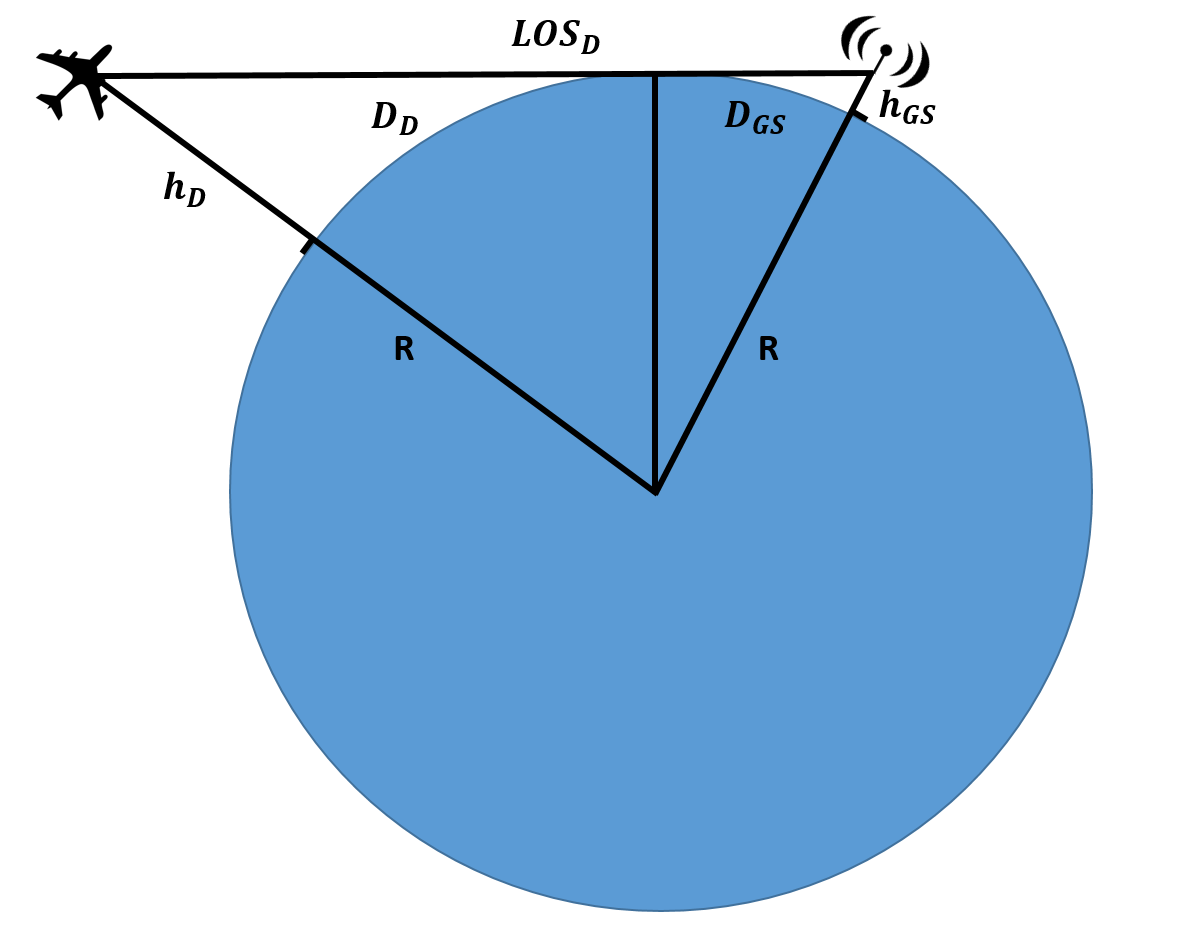
\includegraphics[scale=0.25]{figures/LOS.png}
      \end{figure}
    \end{column}
  \end{columns}

    \begin{align*}      
        LOS_d[km]  \approx {3.57\cdot (\sqrt{h_D[m]} + \sqrt{h_{GS}[m]}} )
    \end{align*}

\end{frame}


\begin{frame}{Telecommunication}{Link Budget}
      \begin{block}{}
        \begin{itemize}
          \item {Accounting of all the gains and losses from the transmitter, through the medium, to the receiver in a telecommunication system.}
          \item {Decisive tool to desing a system and meet the requirements.}
        \end{itemize}
      \end{block}
    \begin{align*}      
        P_{RX} = P_{TX} + G_{TX} - L_{TX} - L_{FS} - L_{M} + G_{RX} - L_{RX}
    \end{align*}
     \begin{itemize}
     \item{\textbf{Free Space Loss}: Loss in signal strength due to traveling in free space, under circustances without obstacles that might cause the signal to be reflected, refracted or additionally attenuated.}
      \end{itemize}

\end{frame}

\begin{frame}{Telecommunication}{Fresnel Zones}
   \begin{block}{}
        \begin{itemize}
          \item {\textbf{Effect of multipath propagation:} Calculate reflections and diffraction in the radio link.}
          \item {Importance of the Fresnel Zone 1: Calculated so that the phase shift of the reflected signal arrives the receiver with 360 degrees phase shift, not affecting the performance.}
          \item {Hard to get 100\% clearance. Rule of thumb: 60\% clearance in Zone 1.}
          \item {The size of the ellipse is determined by the frequency of operation and the distance between the two sites.}
        \end{itemize}
      \end{block}
      \begin{figure}
        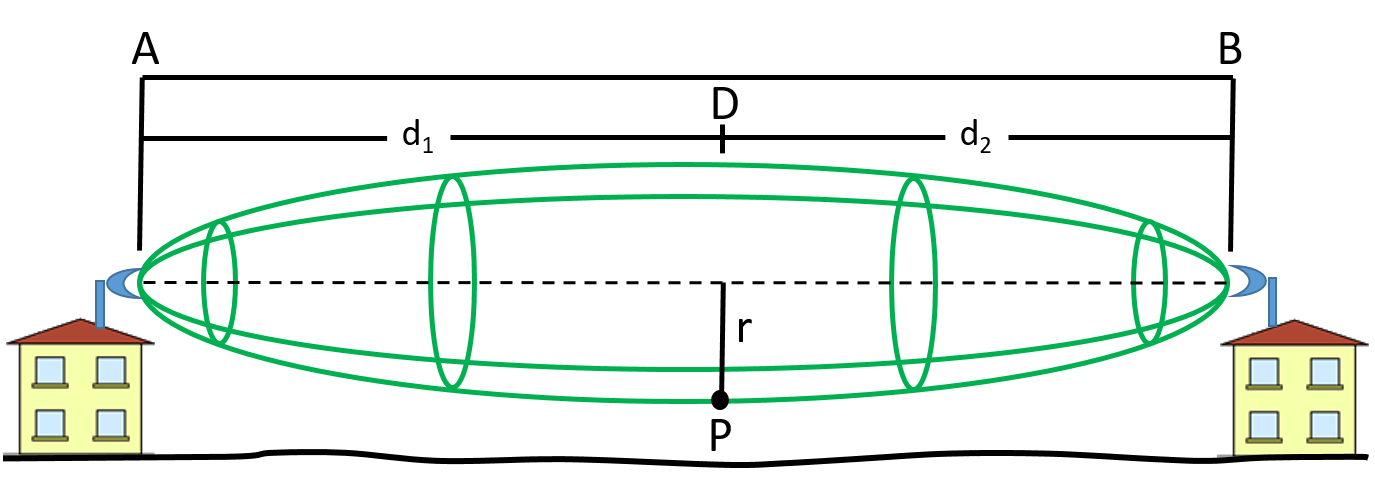
\includegraphics[scale=0.3]{figures/fresnel_zone.png}
      \end{figure}

\end{frame}